\documentclass[tikz,border=3pt]{standalone}
\usepackage[T1]{fontenc}
\usepackage{microtype}
\usepackage{xcolor}
\usetikzlibrary{arrows.meta,backgrounds,calc,fit,matrix,positioning,shapes.geometric}
\definecolor{FigureInk}{HTML}{243447}
\definecolor{FigureMist}{HTML}{E8EEF0}
\definecolor{FigureAccent}{HTML}{176B63}
\tikzset{
  lane/.style={draw=FigureInk!45, fill=FigureMist!50, minimum width=108mm, minimum height=16mm, anchor=west},
  event/.style={draw=FigureInk, fill=white, rounded corners=2pt, minimum width=25mm, minimum height=9mm, align=center, inner sep=4pt},
  flow/.style={-{Stealth[length=2.3mm,width=1.6mm]}, line width=.7pt, draw=FigureInk},
  audit/.style={-{Stealth[length=2.3mm,width=1.6mm]}, line width=.7pt, draw=FigureAccent, dashed},
}
\begin{document}
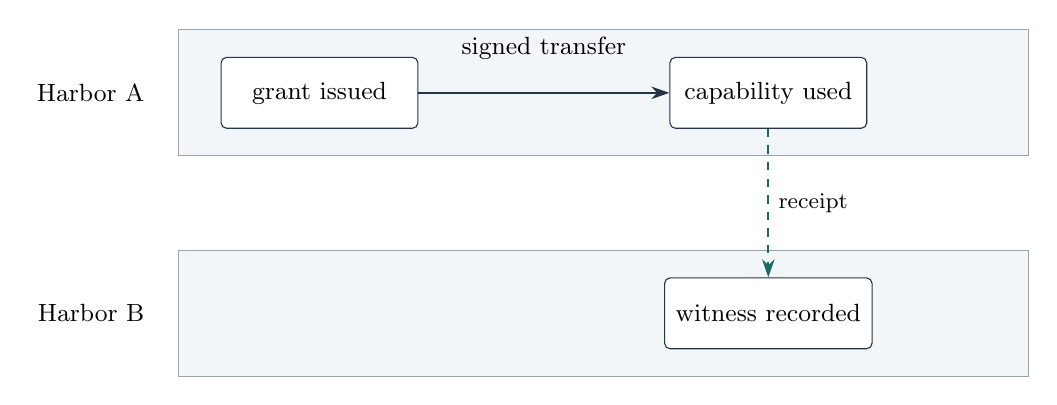
\begin{tikzpicture}[font=\small]
  \node[lane] (a) at (0,1.4) {};
  \node[lane] (b) at (0,-1.4) {};
  \node[anchor=east] at (-.3,1.4) {Harbor A};
  \node[anchor=east] at (-.3,-1.4) {Harbor B};
  \node[event] (grant) at (1.8,1.4) {grant issued};
  \node[event] (accept) at (7.5,1.4) {capability used};
  \node[event] (log) at (7.5,-1.4) {witness recorded};
  \draw[flow] (grant) -- node[above=3mm]{signed transfer} (accept);
  \draw[audit] (accept.south) -- node[right, font=\footnotesize]{receipt} (log.north);
\end{tikzpicture}
\end{document}
